\documentclass{article}
% preamble (Packages importieren)

\newcommand{\comment}[1]{}


\author{Eduard Scherer}
\title{Development \& Construction of an Autonomous Path-Following Drone}
\date{\today}
\usepackage[utf8]{inputenc}

\usepackage[
backend=biber,
style=numeric,
sorting=ynt
]{biblatex}
\addbibresource{references.bib} %Imports bibliography file

\usepackage{graphicx}
\usepackage{parskip}

\usepackage{listings}
\lstdefinestyle{BaselineStyle}
{ %
	commentstyle=\color{Blue},
	keywordstyle=\color{Green},
	numberstyle=\tiny\color{Gray},
	stringstyle=\color{Fuchsia},
	basicstyle=\ttfamily,
	columns=flexible,
	breakatwhitespace=false,
	breaklines=true,
	captionpos=b,
	keepspaces=true,
	numbers=left,
	numbersep=5pt,
	showspaces=false,
	showstringspaces=false,
	showtabs=false,
	tabsize=2,
	xleftmargin=1.5em,
	frame=single,
	framexleftmargin=1.5em
} %
% set to 'BaselineStyle'
\lstset{style=BaselineStyle}



% Dokument
\begin{document}
\maketitle
\tableofcontents
\pagebreak
	\section{Introduction}
	% TODO introduction
	% do at the end of the writing process
	% maybe a quick explanation of the term "drone"
	% drones are being used in war more and more self-built ones(Blheli32 is dead, because of the use in wars.)
	% article about more and more autonomous drones in the Ukraine-Russia War

	\section{Personal Motivation}
	\comment{rather short}
	\section{Literature Review}
	\subsection{General Software Considerations}
	% TODO {why I choose the software (work around the same topic that already exists)}
	
	There are three main softwares to consider when it comes to drones Betaflight, INAV and Ardupilot. All of them are open source. Multiwii was the origin of Betaflight and INAV. Multwii was Arduino based and then upgraded to Baseflight to be able to use the STM32 chips. Then it was forked to Cleanflight, which was later forked again into Betaflight and INAV\cite{history}. 
	
	The following three paragraphs are mostly based on \cite{firmwarearticle} and \cite{firmwarevideo}.
	
	Betaflight is in general the go-to option for first person view drones, commonly known as FPV drones, for either filming or racing. It is the most beginner friendly out of the three, because it has a large community, which results in a wide range of tutorials. When a new board comes out it is normally made to be used with Betaflight. However Betaflight lacks the option for different types of vehicles and generally the automated features are less developed compared to the other two. 
	
	INAV offers basic autonomous flight using waypoints and automated landing. It does not only support quadcopters, but also boats, rovers, planes and wings. It has a similar interface to Betaflight so switching from one to the other is easier than switching to Ardupilot.
	
	Ardupilot basically offers everything the other two have to offer and more for example Submarines and VTOLs. It is not commonly used with FPV, yet you can if you want to. It is more complicated to get into, but as a trade off you will be able to customize everything to your will. It is also the only option for a companion computer like the RaspberryPi. A few years ago it was really expensive to start, because it only supported the Pixhawk family of flight controllers which cost several hundred Franks a piece. However in recent years it has began to support more and cheaper flight controllers.
	
	
	
	
	
	
	\section{Methodology}
	% TODO {(only what has been done + which parts are needed and why I choose them)}
	\subsection{Drone Overview}
	If you want to fly a drone you have two options available either you buy one or you built one. The second option is for people who are interested in tinkering with their electronics until they work, not only the better option but also the cheaper one.
	
	The main parts needed for a drone are the flight controller(Fc), the electronic speed controller(ESC), the receiver, the battery and of course the frame, in addition you can also add a GPS, LEDs and more. The flight controller and electronic speed controller are referred to as Fc and ESC. The Fc runs the chosen software and controls every other part in one way or another. It is directly connected to the ESC, which controls the motors and is connected to the battery. The Fc also communicates with the receiver and GPS if there is one. In my case there is also a RaspberryPi which also connects to the Fc.
	% TODO add a graphic which illustrates the connection between the parts
	  
	\subsection{parts}
	
	\subsubsection[Fc]{Flight Controller}
	There are two different kind of flight controller the All-in-one(AIO) and just a Fc. The AIO is not only a Fc but also the ESC in one piece. This has the advantage of only needing one board instead of two or five. However if only parts of the ESC or the Fc are damaged you need to replace the whole board which is more expensive than replacing only the Fc or ESC. 
	
	Betaflight and INAV both support a wide variety of Fcs compared to Ardupilot which is only supporting a very specific sample of boards\cite{FcSupport}. They have the option of open and closed hardware. Because the open hardware Fcs are quite expensive, so I decided to go with a closed one. The chip used in Fcs is usually a STM32. There are multiple generations of it the mainly used ones are F4, F7 and H7. The F7 and H7 are much faster than the F4 chips so the decision was not that difficult to make. I then decided to go with the Kakute H7 v1.3 (MPU6000)\cite{KakuteH7} from Holybro, because it was ok in the price and available as a stack. It comes shipped with Betaflight so I will need to flash Ardupilot. 

	\subsubsection[ESC]{Electronic Speed Controler}
	%TODO ESC 
	There are two different kind of ESCs, 4in1 and single ESCs. If you use single ESCs you will need one for each motor instead of a single board for all of them. The advantage of 4in1 ESCs is that you do not need a power distribution board, because it is already incorporated in the ESC, and that it can come in a stack. A stack is a Fc and ESC mounted on top of each other. It normally comes with stack screws. The disadvantage is that if a part of the ESC is damaged you need to replace the whole board. What needs to be looked upon buying a ESC is that the peak current of the motor is not higher than the burst current of the ESC, because it could damage a two high current could damage the ESC.
	
	My decision was to go with a 4in1 on a stack, because it is slightly cheaper and normally easier to wire. The only option with the Kakute H7 was the stack with the Tekko32 4in1 with a continuous current of either 50, 60 or 65 Ampere. I chose the 50A\cite{Tekko32} one, because you do not need a high continuous current rating when flying rather slowly and the motors I chose have a peak current of around 42A. 
	
	At the time I bought the ESC it was still shipped with BLHeli32 which as mentioned has seized their operations. I could however flash AM32 onto it.

	\subsubsection{Motor}
	There are two types of motor brushed and brushless ones. The difference between the two types is that the brushed motors are mechanically driven and the brushless motors are electrically driven. Therefor brushless motors also need an ESC to function compared to brushed ones. Brushed motors are used in really small drones with 1S batteries. However even in the small drones brushless motors are the more popular choice\cite{brush/lessmotors}. 
	
	The numbers that are seen on the motors like 2207 are describing the stator of the motor itself. In the case of a 2207 that would be 22mm diameter and a height of 7mm. The usual stator sizes of 5 inch drones are either 2207 or 2306. There is also the KV value which has to be considered. The KV value is the number of revolutions per minute(rpm) a motor turns when one volt is applied. The lower the KV value the more efficient is the motor and the higher the KV value the more responsive it is. The KV value for a 5 inch drone with a 4S battery is between 2300 and 2800. I chose the Iflight Xing-E Pro 2207\cite{xingepro} with a KV value of 2450, because the IFlight-Xing motors are known to be of good quality. 
	% TODO get a new brush/brushless motor picture
%\begin{figure}
%	\centering
%	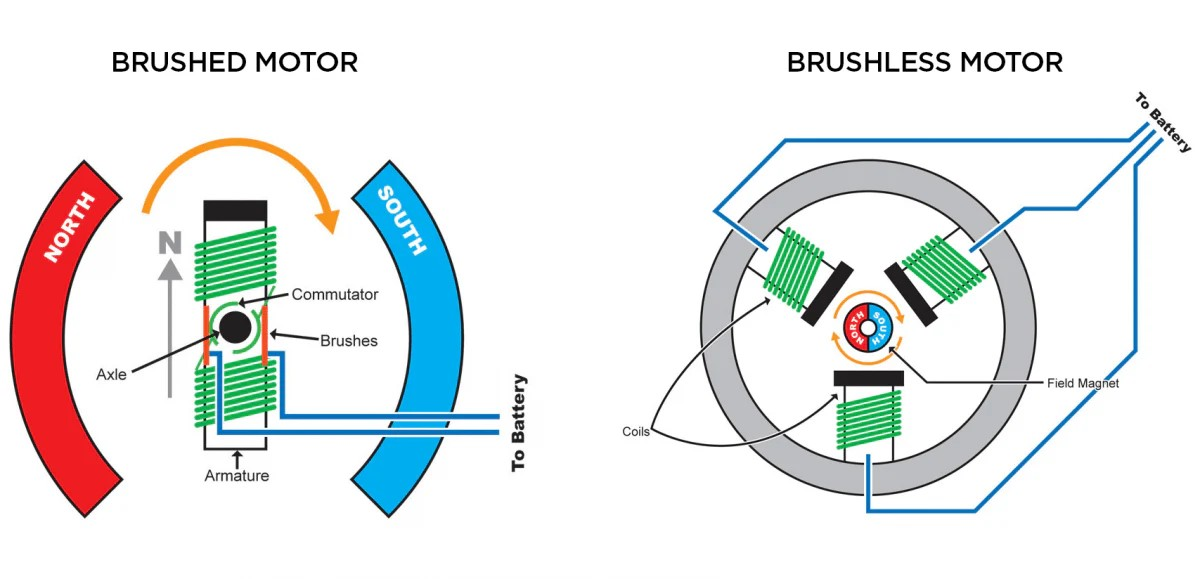
\includegraphics[0.5]{pictures/motor}
%	\caption{\cite{picturemotor}}
%	\label{fig:motor}
%\end{figure}
	
	\subsubsection{Battery}
	There are two main types of batteries lithium polymer(LiPO) and Lithium-ion(Li-ion) batteries. LiPo batteries have a tendency to go up in flames by themselves. They have compared to the Li-ion batteries a much higher discharge rate, also seen as C value, so they are well suited for racing drones. However Li-ion batteries have a higher energy density, which means that they can store more mAh with the same weight as LiPo batteries, so they are more used in long range flying. The batteries have normally multiple cells, for example a 4S LiPo batterie contains 4 cells. This is important, because the more cells you have the higher is the voltage and so you will need a motor with a lower KV value. 
	
	I first wanted to buy two Li-ion battery packs, however they are firstly hard to get and secondly much more expensive. The other option would have been to solder them together myself, but it requires some soldering skill, which I did not have then. So I decided to go with 4S LiPo batteries from the Tattu R-line with 120C and 2000mAh\cite{tattu}, because I want something that can fly longer than just three or four minutes. I chose the brand Tattu, because it was the only known brand that was on AliExpress from where I got all the other components, so it seemed to be easier to also chose a battery from there. 
	
	\subsubsection{GNSS(Global Navigation Satellite System)/Compass}
	% TODO GNSS/Compass
	
	Micro M10 from Holybro choosen, because it is from the same manufacturer as the Fc.
	4 Concurrent GPS
	CEP of 2 m(short explanation box)
	connects via Uart
	\\ built-in compass connects to the Fc with a I2C protocol...
	
	
	

	\subsubsection{Transmitter Protocols}
	
	\subsubsection*{Frsky}
	\subsubsection*{Crossfire TX}
	\subsubsection*{Elrs}
	\subsubsection*{mLrs}
	
	\subsubsection{Data Transfer Protocols}
	\subsubsection*{SPI}
	\subsubsection*{Uart}
	\subsubsection*{I2C}
	
	\subsubsection{Radio/Transmitter}
	%TODO Radio/Transmitter
	you can play games on the Boxer Radio
		

	\subsubsection{Smoke Stopper}
	A part that stops the ESC from short circuiting due to wrongly soldered parts. It is there to prevent the part getting destroyed. There are two groups of it one that you buy and gets destroyed when the ESC short circuits instead of the ESC and it saves you money by not destroying the ESC and sacrificing itself. There is another category that does not destroy itself and there are also some that you can solder together on your own. These work by using a lamp(Glühbirne).
	
	\subsubsection{Problems with the Parts}

	There were two problems that arose one less severe than the other. One problem was that my ordered Kakute-Tekko stack did not include stack screws, which they normally do. Stack screws are just screws that you can use to mount the stack onto the frame. So I needed to purchase them separately.
	
	The more severe problem I ran into was that the batteries from AliExpress were first hold by the swiss border control and then I received two insect traps instead of batteries. Luckily I ordered one of the same batteries from Conrad, because the other two took too long to deliver. 
	
	
	
	\subsection{soldering}
	
	\subsection{ardupilot}
	The following is based on the ArduPilot copter documentation\cite{ardupilotdocs}.
	\subsubsection{Ground Station}
	To configure ArduPilot there are multiple softwares so called ground stations(GCS) required. They are normally ground-based and can transmit data via with a wireless telemetry device or USB cable.  With the telemetry device they can also control the drone from the ground and alter the route it is autonomously flying. 
	
	The most widely used GCS is Mission Planner(MP)\cite{MissionPlanner} it is widely used, but runs only on Windows and Mac OS. It also has a wiki which helps you install it. I will use it for the first-time configuration of my drone. 
	
	Another GCS is MavProxy it is based on Python and is only for the Linux operation system(OS). Which is the OS I will have on my RaspberryPi companion computer. 
	
	There is also QGroundContrlol which is unique, because it supports next to Windows, Mac OS and Linux also Android and IOS.

	\subsection{Firmware Installation}
	
	For the first time installation I need to flash the Kakute H7 with ArduPilot, because it is shipped with Betaflight as mentioned earlier on. For that I downloaded the ArduPilot firmware\cite{ArduPilotFirmware} for the Kakute H7. Afterwards the STM32CubeProgrammer\cite{STM32CubeProgrammer}, to flash the firmware onto the Fc. I connected the Fc in DFU mode directly with the computer using a USB cable. Then selected the USB port with which the Fc is connected and flashed the Fc. A reboot to get out of the DFU mode was required before connecting the Fc to MP and saw the first Yaw measurements. The progress of flashing the firmware was straight forward which will not be the case for the rest of the configuration. 
	% TODO add an explanation box for the DFU mode.
	% TODO add pictures of Yaw measurement.

	\subsubsection{GPS Connection}
	When I tried to get a GPS connection a No GPS message appeared. Changing the \lstinline|GPS_Type = 2| for the Ublox GPS did not change the No GPS error message.
	
	%TODO add picture No_GPS
	Even though I was certain that the GPS worked well, because the compass of the GPS was already detected in the compass calibration tab.
	
	% TODO add picture compass_detected
	I then went outside, away from metal tables and as far away from my computer that was possible with the USB cable it still did not show up in MP. I also checked the soldering and if the cables from the GPS to the Fc are connected correctly and both seemed fine. The GPS itself was not damaged, because the blue led was blinking constantly which means it is connecting to a GNSS.

	The problem was that the \lstinline|Serial3_Protocol|(Which is for the Uart3, which will be used for the connection to the RaspberryPi) was set to 5 which means GPS, however by being on 5 it blocked the Uart4, to which my GPS was really connected. After disabling the Uart3 it finally worked.
	
	The GPS is quite precise outside.
	%TODO insert picture GPS_Outside
	
	It also works sometimes inside and is precisely on my room, but sometimes it shows that I'm in Poland the middle of the Atlantic Ocean or Iceland.
	%TODO insert pictures GPS_Inside1/2
	 
	\subsubsection{Receiver/Transmitter}
	changing RC\_optopns to 420 k baudrate for Elrs
	\\ connection between the receiver and radio exist... radio says telemetry recovered and receiver isn't flashing a green light anymore, but has a constant blue light. However no connection to Fc yet.
	\\ followed the page (reference to expresslrs.org page) it does not work yet. 
	\\ could change the receiver to the uart1 which is usually for the receiver, but it would require an JHSt thingy and more soldering
	\\
	\\ it works now... I needed to set Brd\_Alt\_Config to 1, which is a Fc specific parameter and I found it in the kakute H7 section which said that it needed to be done
	\subsubsection*{Battery/Servos/Smoke Stopper/Compass Calibration}
	pluging in battery with smoke stopper attached, smoke stopper does not light up
	\\changing the battery settings for the tekko32 F4 4 in 1 Esc as explained in the kakute h7 fc page of ardupilot only needed to change the BATT\_MONITOR ot 4 all the others were already correct, I can see now the voltage and the Amperage of the battery
	\\the only thing missing before I can arm it is the compass calibration...(note: I'm inside so the GNSS has no connection but it works as soon as I get under the free sky.)
	\\ compass calibration fails multiple times.. even tried changing it as the docs from holybro suggest compass\_ortient= 6 still does not work. 
	\\ turns out you need good GPS lock to do it...I'm inside
	\\with GPS lock and outside with relaxed settings and both compass\_orient =6 and 0 it does not work
	the failure could be caused by the computer which is nearby or the table which is metal on which I've done it. 
	There could also be the fix by doing the largevehicle Magcal, which helped a person online who also had a 5 inch copter. 
	\\ somehow it calibrated??? I tried to calibrate it multiple times in different settings and it never worked and without even being able to finish my last try at calibration it worked??? it might have been the largevehical magcal that has done it...
	\\
	\\ Motor testing works after connecting assigning the right position to the motors and setting the mot\_pwm\_type to dshot 600
	\\new error message: battery failsafe, begins to continously beep(but not always???) might be caused from the connection to the computer... so that it will take the wrong power input as main power
	\\ the motors suddenly began to beep I have no idea why
	\\ I got the error compass variance, but when I move further away from my computer it goes away.
	\\ all prearm checks are gone now except magfield
	\\ magfield problems went away after positioning the drone further away from the computer... now there is no prearm check(you can also disable them by setting arming\_check to 0) that needs to be done and I can arm the drone
	\\ only problem is that I don't now how... I was able to assign the rc channel 5 to it. 
	\\ disabling arming check... however the MAV rejects the forece arm command. 
	\\ arming worked via radio and MP after I disabled the Geofence that I put in somewhen earlier, even though I disabled arming\_check the geofence did not get disabled.
	\\ I can do it without mission planner, but the Fc does not get any power from the esc... it might be, because I have connection between the Fc and Esc in the second slot. It was only a bad connection between the Fc and ESC nothing about the slot I put them in. 
	\\ bench testing with propellers... I hit one of the receiver antennas with a prop it fell off I was able to easily attach it again, however I'm not sure if that particular antenna is working now
	\\ new prearm error crashdump bin detected, so through my research I've concluded that the error is currently insignificant, because it was probably caused through my bench testing.
	\\ I was not able to get rid off the error and I will analyse the crash dump file later on somewhen. I just did all the prearm checks except crash dump bin detected and then disabled prearm checks. 
	\\ the drone flew, even though it was only spinning in one direction because two motors currrently spin in the wrong direction.
	\\ the reverse button in MP is not working
	\\ to reverse the motors I need to set servo\_blh\_auto to one and open it in Blhelisuite32\cite{BLHeliSuite32}. By using the reversed mode in Blhelisuite32 I was able to reverse one motor but one that should not be reversed. After trying multiple times I now finally got the A and C motor spinning counter clockwise. 
	\\ it flew really shaky after disabling the arming\_check again it might really be a compass problem again.
	\\ the compass calibration worked correctly after I took the GPS module and put it directly onto the flight controller instead of having it on the frame
	\\ again trying to fly shaking violently and somewhat crashing into the ground.
	\\ tightening everything on the quad... might work
	\\ I tightened everything tried different props, due to damage on the first set and possiblity of inbalanced props in the second set, it still wobbled extremely. 
	\\ then I came to the conclusion through different websites that my PID values are wrong and it turns out they actually were and I needed to change my parameters from a 9 inch drone to a 5 inch.
	\\ it flew well, however I still need to invert the switches from the radio, because it currently goes into the wrong direction when I steer left it goes right and vice versa. 
	
	
	
	
	
	\section{Results}
	\section{Discussion and Outlook}
	\section{Conclusion}
	
	\section{References}
	\printbibliography[
	heading=bibintoc,
	title={Bibliography}
	]	
	\section{Table of Figures}
	\comment{(short table on which every figure description with the page number is listed)}
\end{document}
